\documentclass[]{../project_report}
\author{%
	Marcin Lembke\\
	\texttt{\href{mailto:M.Lembke@stud.elka.pw.edu.pl}%
			{\nolinkurl{M.Lembke@stud.elka.pw.edu.pl}}}
	\and
	Marcin Malesa\\
	\texttt{\href{mailto:M.Malesa@stud.elka.pw.edu.pl}%
			{\nolinkurl{M.Malesa@stud.elka.pw.edu.pl}}}
}
\supervisor{dr inż. Piotr Bilski}
\title{Algorytm przeszukiwania z tabu do rozwiązywania układanki Sudoku (PB5)}
\subtitle{Sprawozdanie wstępne}
\course{Współczesne metody heurystyczne}
\coursecode{WMH}
\university{Politechnika Warszawska}
\faculty{Wydział Elektroniki i Technik Informacyjnych}

\begin{document}
	\maketitle

	\section{Sudoku}
	Sudoku to gra logiczna, której celem jest uzupełnienie planszy, zazwyczaj o rozmiarze 9 na 9 pól, w taki sposób aby w każdym wierszu, kolumnie oraz wyznaczonym bloku 3 na 3 pola, znalazło się po jednej cyfrze z zakresu 1 do 9.
	
	\begin{figure}[H]
		\centering
		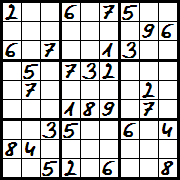
\includegraphics[scale=0.75]{sudoku_example.png}
		\caption{Przykładowa plansza Sudoku. Pogrubionymi liniami oznaczono bloki o rozmiarze 3 na 3 pola. Źródło: \href{https://upload.wikimedia.org/wikipedia/commons/2/2d/Sudoku_przyklad.png}{wikimedia.org}}
	\end{figure}
	
	\section{Przeszukiwanie tabu}
	Przeszukiwanie tabu (ang. \textit{Tabu search}, TS) to metaheurystyka wykorzystywania wraz z metodami przeszukiwania przy problemach optymalizacyjnych.
	
	Ideą algorytmu jest iteracyjne przeszukiwanie przestrzeni wszystkich możliwych rozwiązań. Przy każdym ruchu korzysta się z tak zwanej listy tabu (ang. \textit{Tabu list}).
	
	\section{Problemy do rozwiązania i wstępne rozwiązania}
	Analizując zadanie zaprojektowania i implementacji algorytmu do rozwiązywania łamigłówki Sudoku wykorzystujący przeszukiwanie tabu można dostrzec pewne podstawowe problemy:
	
	\begin{enumerate}
		\item Jak generować plansze do testowania -- liczba możliwych (rozwiązanych) plansz to ponad \(6,67 \cdot 10^{21}\). Ponadto liczba plansz dających się jednoznacznie rozwiązać wynosi ponad 49 tys. dla 17 uzupełnionych pól.
		
		Problem można przedstawić następująco: w jaki sposób wygenerować planszę do Sudoku dającą się jednoznacznie rozwiązać i jak
	\end{enumerate}
	
	\section{Podsumowanie}
\end{document}
